\section{Auswertung}
\label{sec:Auswertung}

%\section{Fehlerrechnung}
\label{subsec:fehlerrechnung}

\subsubsection{Mittelwert}
\begin{equation}
\overline{v} = \frac{1}{N} \sum_{i=1}^N v_i
\end{equation}

\subsubsection{Standardabweichung}
\begin{equation}
s_i = \sqrt{\frac{1}{N - 1} \sum_{j=1}^N \left(v_j - \overline{v}\right){^2}}
\end{equation}

wobei $v_j$ ($j = 1, ..., N$) die Messwerte sind.

\subsubsection{Streuung der Mittelwerte}
\begin{equation}
\sigma_i = \frac{s_i}{\sqrt{N}} = \sqrt{\frac{\sum_{j=1}^N \left(v_j - \overline{v_i}\right){^2}}{N \left(N - 1 \right)}}
\end{equation}

\subsubsection{Gaußfehler}
Bei einer fehlerbehafteten Funktion $f$ mit $k$ als fehlerbehafteter Größe und $\sigma_k$ als Ungenauigkeit, gilt:

\begin{equation}
\Delta x_k = \frac{\mathrm{d}f}{\mathrm{d}k}\sigma_k
\end{equation}.

 Der relative Gaußfehler berechnet sich nach:
\begin{equation}
\Delta x_\text{k, rel} = 1 \pm \frac{\Delta x_k}{|x|}\cdot 100\%
\end{equation}.

Der absolute Gaußfehler ergibt sich aus:
\begin{equation}
\Delta x_i = \sqrt{\left(\frac{\mathrm{d}f}{\mathrm{d}k_{1}}\cdot \sigma_{k_{1}}\right)^2 + \left(\frac{\mathrm{d}f}{\mathrm{d}k_{2}}\cdot \sigma_{k_{2}}\right)^2 + ...}
\end{equation}.


\subsection{Auf- und Entladevorgang}
\label{sec:a}
Die Zeitkonstante $\tau = RC$ eines RC-Kreises wird Anhand der Auf-/Entladekurve bestimmt. Dazu wird ein Stromkreis wie in Abb. \ref{fig:rc-kreis} genutzt, wobei $U_C$ mit einem digitalen Speicheroszilloskop gemessen wird. Der gemessene Spannungsverlauf findet sich in Abb. \ref{fig:entladekurve}.
\begin{figure}
  \centering
  \includegraphics{build/a1.pdf}
  \caption{Verlauf der Kondensatorspannung $U_C$ bei angelegter Rechteckspannung am RC-Kreis. Zur Bestimmung der Zeitkonstante wird der mit den schwarzen vertikalen Linien markierte Zeitbereich genutzt.}
  \label{fig:entladekurve}
\end{figure}
Zur Auswertung wird nun das Spannungsoffset
\begin{equation}
  U_0 = \SI{-5.6}{\volt}
\end{equation}
korrigiert, die Messwerte logarithmiert und mittels linearer Regression die Steigung einer Ausgleichsgeraden ermittelt. Aus (\ref{a}) folgt über
\begin{align}
  U (t) &= U (0) \cdot \symup{e}^{\sfrac{-t}{RC}}\\
  \ln{U(t)} &= \ln{(U (0) \cdot \symup{e}^{\sfrac{-t}{RC}})} \\
  \ln{U(t)} &= \ln{U (0)} - \frac{1}{RC} \cdot t
\end{align}

, dass

\begin{equation}
  RC = -\frac{1}{a}
\end{equation}

ist, mit der Steigung $a$ der Ausgleichsgeraden. Die logarithmierten Messwerte über die Zeit aufgetragen finden sich in Abb. \ref{fig:auswertung_a}, das Ergebnis lautet
\begin{equation}
  RC = \SI{1.360+-0.001}{\milli\second}
\end{equation}
%\begin{table}
%  \centering
%  \caption{Ergebnis der Auswertung der Zeitkonstante des RC-Kreises.}
%  \label{tab:ergebnis_a}
%  \sisetup{
%    round-mode=figures
%  }
%  \begin{tabular}{
%    l@{}
%    S[table-format=1.3e2, round-precision=4] @{${}\pm{}$} S[table-format=1.2e2, round-precision=3]
%  }
%    \toprule
%    & \multicolumn{2}{c}{RC / \si{\second}} \\
%    \midrule
%    \begin{table}
        \caption{Messergebnisse aus dem A-Scan. Neben den abgelesenen und berechneten Daten $d_n$ sind auch die zuvor mittels Messschieber bestimmten Abmessungen $d_n^\text{mech}$ eingetragen.}
        \centering
        \label{tab:a}
        \begin{tabular}{l@{}S[round-mode=off, table-format=2.0]S[table-format=2.3, round-precision=4, round-mode=off] S[table-format=2.2, round-precision=4, round-mode=figures] S[table-format=1.4, round-precision=4, round-mode=figures] S[table-format=2.3, round-precision=4, round-mode=figures] S[table-format=2.2, round-precision=4, round-mode=figures] S[table-format=2.4, round-precision=4, round-mode=off] } \toprule & {$\text{Störstelle}$}& {$d_1/\si{mm}$}& {$d_2/\si{mm}$}& {$2r/\si{mm}$}& {$d_1^\text{mech}/\si{mm}$}& {$d_2^\text{mech}/\si{mm}$}& {$2r^\text{mech}/\si{mm}$}\\\midrule
& 1 & 18.02 & 61.56149999999999522515 & 0.46050000000000257394 & 19.62000000000000099476 & 59.61999999999999744205 & 0.80 \\
& 2 & 19.93 & 59.78699999999999192823 & 0.32400000000000828138 & 17.76000000000000156319 & 61.29999999999999715783 & 0.98 \\
& 3 & 61.29 & 13.78650000000000019895 & 4.96500000000000429878 & 61.28000000000000113687 & 13.43999999999999950262 & 5.32 \\
& 4 & 54.05 & 22.11299999999999599254 & 3.87300000000000821387 & 53.84000000000000341061 & 21.69999999999999928946 & 4.50 \\
& 5 & 46.68 & 30.43950000000000244427 & 2.91749999999998976818 & 46.50000000000000000000 & 30.07999999999999829470 & 3.46 \\
& 6 & 39.04 & 39.03900000000000147793 & 1.96199999999999152855 & 38.60000000000000142109 & 38.71999999999999886313 & 2.72 \\
& 7 & 31.12 & 47.09249999999999403144 & 1.82550000000000767209 & 30.82000000000000028422 & 46.88000000000000255795 & 2.34 \\
& 8 & 23.07 & 55.14600000000000079581 & 1.82550000000000411937 & 22.78000000000000113687 & 54.82000000000000028422 & 2.44 \\
& 9 & 15.01 & 62.92650000000001142553 & 2.09849999999999115019 & 14.82000000000000028422 & 62.97999999999999687361 & 2.24 \\
& 10 & 7.23 & 70.98000000000000397904 & 1.82549999999999990052 & 6.87999999999999989342 & 70.79999999999999715783 & 2.36 \\
& 11 & 55.82 & 15.42450000000000009948 & 8.78699999999999548095 & 55.11999999999999744205 & 14.63000000000000078160 & 10.29 \\
 \bottomrule \end{tabular} \end{table}

%    \bottomrule
%  \end{tabular}
%\end{table}

\begin{figure}
  \centering
  \includegraphics{build/a2.pdf}
  \caption{Logarithmierter Kondensatorspannungsverlauf mit Ausgleichsgerade. Fehlerbalken wurden zur Verbesserung der Lesbarkeit ausgelassen.}
  \label{fig:auswertung_a}
\end{figure}

\subsection{Schwingungsverhalten}
\label{sec:b}
Nun soll die Zeitkonstante auf andere Art und Weise ermittelt werden, undzwar dadurch, dass eine Wechselspannung an den RC-Kreis angelegt wird und dabei die resultierende Spannung bzw. Phasenverschiebung gemessen wird. Der Aufbau der Schaltung findet sich an Abb. \ref{fig:phase-frequenz}. Hierbei wird die Zeitkonstante mittels nichtlinearer Ausgleichsrechnung an die der Formeln (\ref{eqn:amplitude}) und (\ref{eqn:phase}) bestimmt. Die Ergebnisse finden sich in Tabelle \ref{tab:ergebnis_b} und Abb. \ref{fig:auswertung_b1}/\ref{fig:auswertung_b2}.

\begin{table}
  \centering
  \caption{Ergebnis der Auswertung der Zeitkonstante des RC-Kreises.}
  \label{tab:ergebnis_b}
  \sisetup{
    round-mode=figures
  }
  \begin{tabular}{
    l
    S[table-format=1.2e2, round-precision=3] @{${}\pm{}$} S[table-format=1.0e2, round-precision=1]
  }
    \toprule
    & \multicolumn{2}{c}{RC / \si{\second}} \\
    \midrule
    Messreihe Amplitude \input{build/b1.txt}
    Messreihe Phasenverschiebung \input{build/b2.txt}
    \bottomrule
  \end{tabular}
\end{table}

\begin{figure}
  \centering
  \includegraphics{build/b1.pdf}
  \caption{Frequenzabhängigkeit des Verhältnisses der Amplitude am Kondensator zur angelegten Amplitude, einfachlogarithmische Darstellung.}
  \label{fig:auswertung_b1}
\end{figure}

\begin{figure}
  \centering
  \includegraphics{build/b2.pdf}
  \caption{Frequenzabhängigkeit der Phasenverschiebung von Kondensator- und Generatorspannung, einfachlogarithmische Darstellung.}
  \label{fig:auswertung_b2}
\end{figure}

\newpage
\subsection{Integrator}
\label{sec:c}
Bei ausreichend hohen Frequenzen $\omega \gg \sfrac{1}{RC}$ kann ein RC-Kreis als Integrationsglied verwendet werden. Die hochfrequenten Anteile der angelegten Spannung werden dabei aufintegriert. Einige Beispiele dazu finden sich in den Abbildungen \ref{fig:d1}, \ref{fig:d2} und \ref{fig:d3}.

\begin{figure}
  \centering
  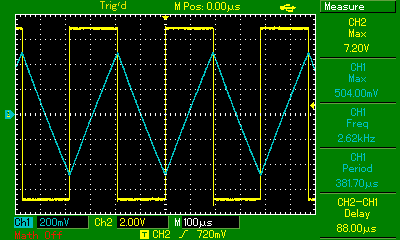
\includegraphics[scale=0.8]{daten/d/MAP004.png}
  \caption{Spannungsverlauf einer Dreiecksschwingung und der vom RC-Kreis integrierten resultierenden Parabelschwingung.}
  \label{fig:d1}
\end{figure}

\begin{figure}
  \centering
  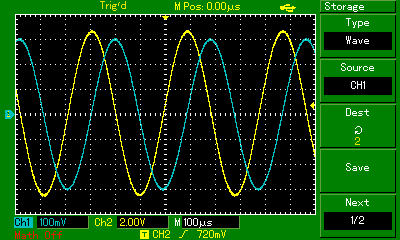
\includegraphics[scale=0.8]{daten/d/MAP005.png}
  \caption{Spannungsverlauf einer Rechteckschwingung und der vom RC-Kreis integrierten resultierenden Dreieckschwingung.}
  \label{fig:d2}
\end{figure}

\begin{figure}
  \centering
  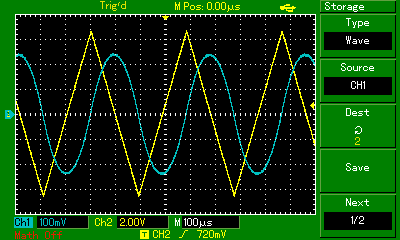
\includegraphics[scale=0.8]{daten/d/MAP006.png}
  \caption{Spannungsverlauf einer Sinusschwingung und der vom RC-Kreis integrierten resultierenden Cosinusschwingung.}
  \label{fig:d3}
\end{figure}

\subsection{Messdaten}
Die Angabe der Oszilloskop-Messdaten aus \ref{sec:a} ist aufgrund der Menge (6000 Punkte) nicht möglich. Die restlichen Daten finden sich in Tabelle \ref{tab:daten}.

\begin{table}
  \centering
  \caption{Messdaten.}
  \label{tab:daten}
  \sisetup{
    round-mode=figures
  }
  \begin{tabular}{
      l@{}
      S[table-format=5.0]
      S[table-format=1.3]
      S[table-format=1.1]
      S[round-precision=3, table-format=1.4] @{${}\pm{}$} S[round-precision=2, table-format=1.5]
      S[table-format=1.2]
      S[round-precision=3, table-format=1.4] @{${}\pm{}$} S[round-precision=2, table-format=1.4]
    }
    \toprule
    & {$f / \si{\hertz}$} & {$U/ \si{\volt}$} & {$U_0 / \si{\volt}$} & \multicolumn{2}{c}{A} & {$a / \si{\milli\second}$} & \multicolumn{2}{c}{$\phi / \si{\radian}$}\\
    \midrule
    \input{build/daten.txt}
    \midrule
    &\multicolumn{8}{c}{
      $\Delta U^\text{rel} = 5\%, \quad \Delta U_0^\text{rel} = 5\%, \quad \Delta a^\text{rel} = 5\%$
    }\\
    \bottomrule
  \end{tabular}
\end{table}
